%========= Method overview
%% trim=left bottom right top
\newcommand{\MethodOverview}{
\begin{figure}[t]
    \centering
    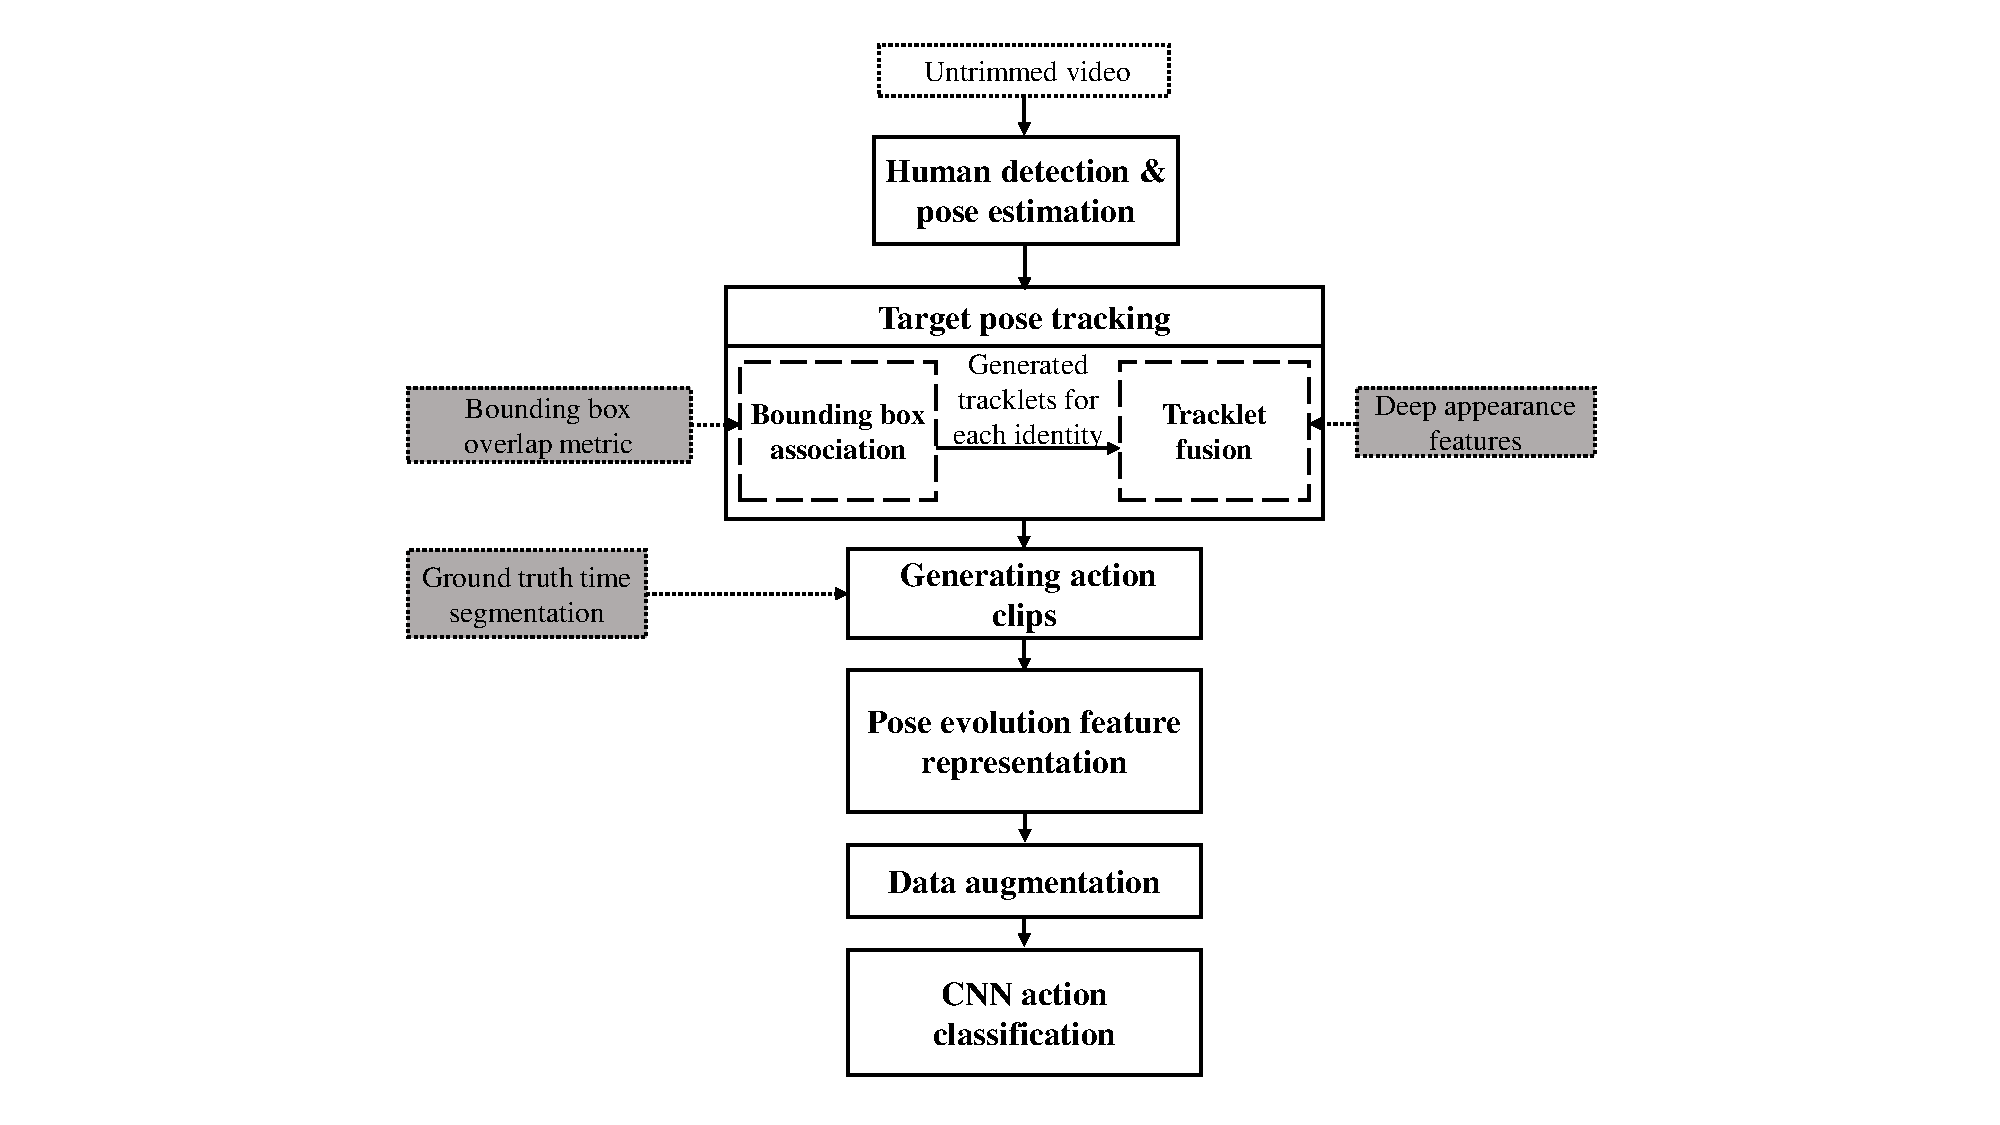
\includegraphics[width=1\linewidth, trim=2.5in 0.0in 2.5in 0.0in, clip=true]{Figures/Method.pdf}
    \caption{Overview of the proposed multi-stage method for human behavior phenotyping in untrimmed videos. At the first stage, human detection and pose estimation is applied on the recorded video. At the second stage, the regressed bounding boxes for each detected person and corresponding keypoints are used for the tracking the identities in video. Tracking is done in an incremental process incorporating both appearance and time information. Outputs of tracking the target identity along with ground-truth time segmentation are used for generating a compact representation of the target actor pose evolution in time for each action clip. Finally, the augmented pose evolution representation is fed to a CNN-based action classification network to recognize actions of interest.}
    \label{fig:Method}
    \vspace{-.1in}
\end{figure}
}
%===============================
\newcommand{\PoseNet}{
\begin{figure*}[ht]
    \centering
    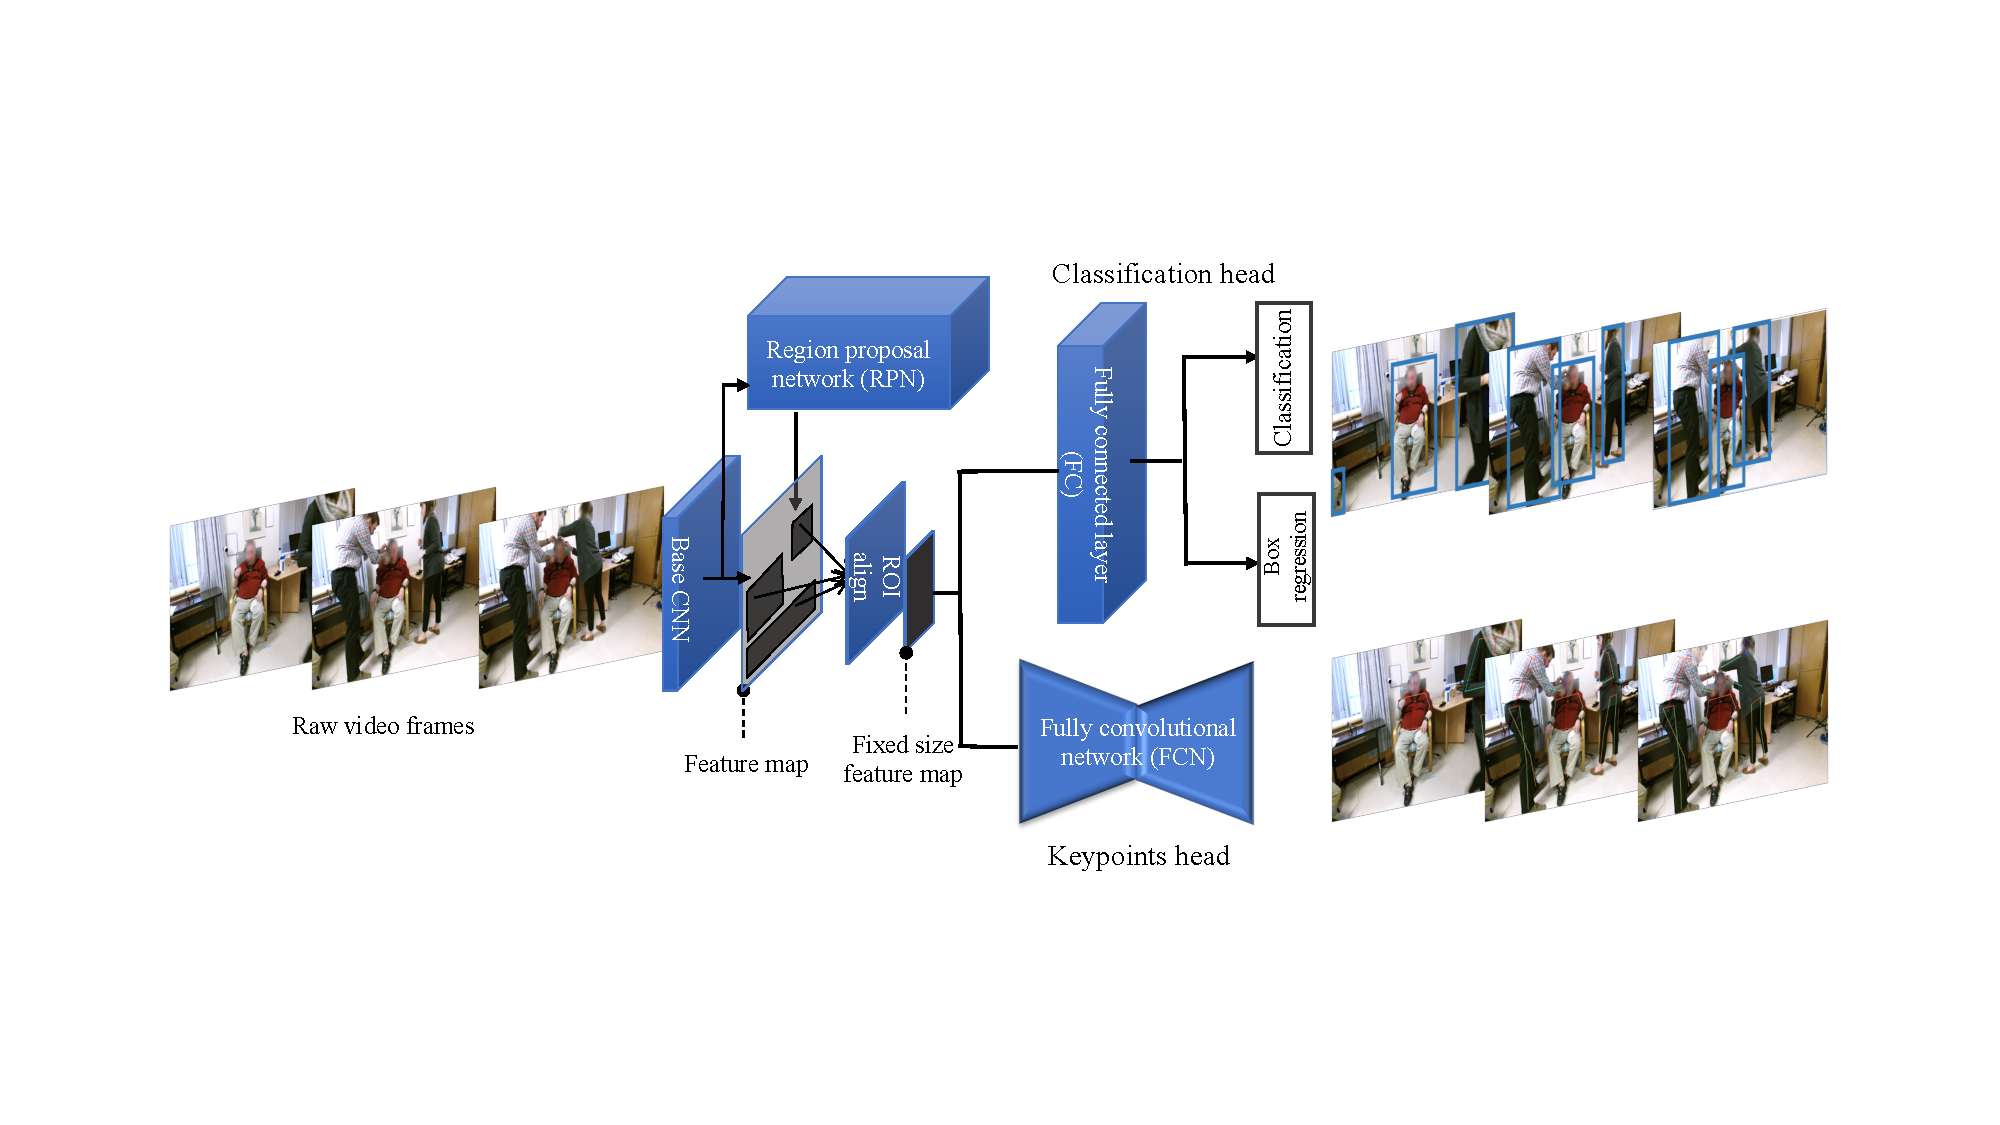
\includegraphics[width=0.9\textwidth, trim=1.1in 1.6in 1.1in 1.6in, clip=true]{Figures/PoseNet.pdf}
    \caption{Architecture of the pose estimation network. Each video frame is fed separately to the base network (ResNet 101) for feature extraction. A region proposal network is applied on the output feature map to find the areas with the highest objectness probability. The fixed size features for proposed regions are then given to the classification and pose estimation heads to find the human bounding boxes and their corresponding keypoints.}
    \label{fig:Pose}
    \vspace{-.1in}
\end{figure*}
}
%====================================
\newcommand{\Tracking}{
\begin{figure*}[t]
    \centering
    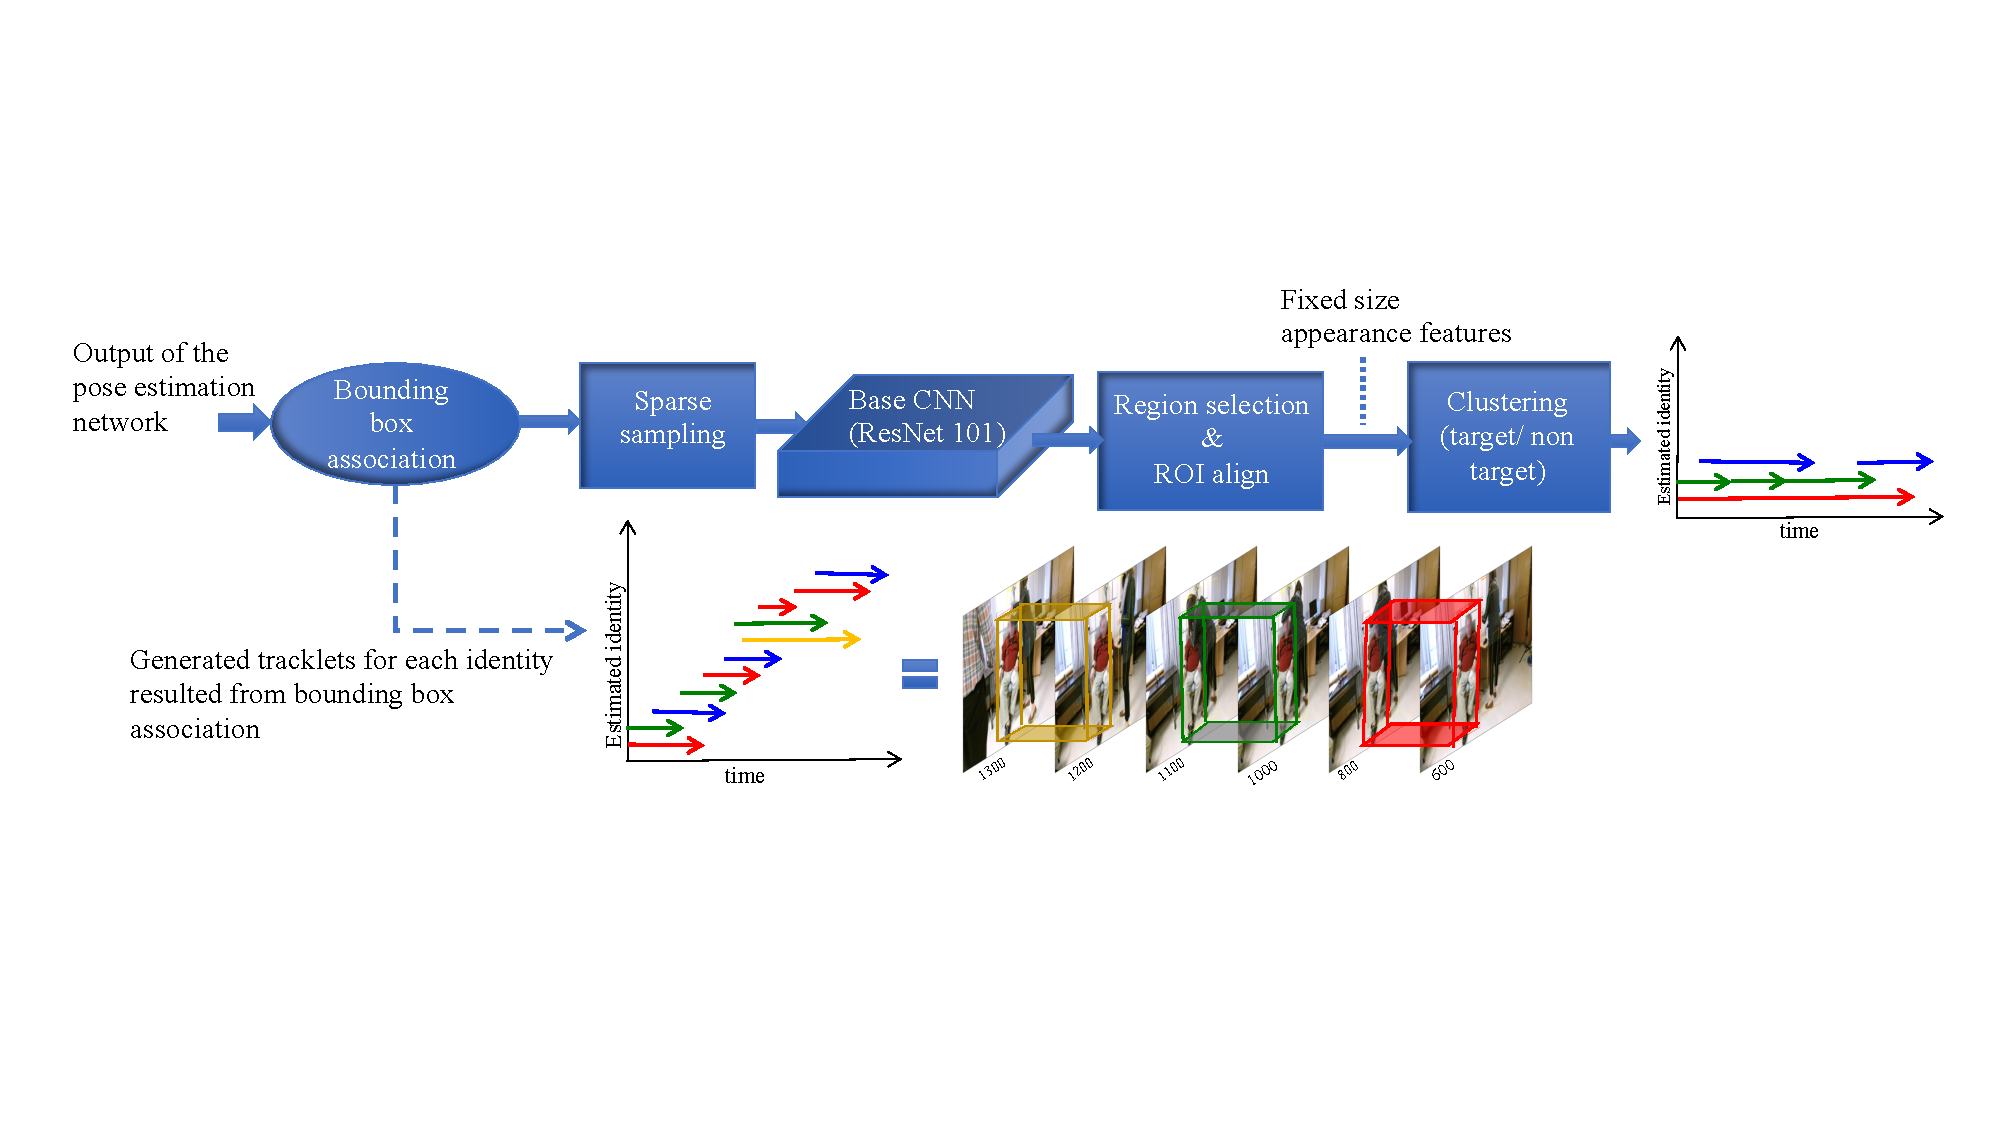
\includegraphics[width=0.9\textwidth, trim=0.1in 2.0in 0.1in 1.8in, clip=true]{Figures/Tracking.pdf}
    \caption{Hierarchical pose tracking using temporal and appearance features. Tracking starts by associating detected bounding boxes in each pair of consecutive frames using the intersection over union metric. Output of this step is a number of different tracklets for each identity. At the next step generated tracklets are pruned based on their length, and pose estimation confidence followed by sparse sampling. Finally, generated tracklets which belong to the target identity are merged according to their appearance similarity to create the endpoint track for the target human actor (best viewed in color).}
    \label{fig:Tracking}
    \vspace{-.1in}
\end{figure*}
}
%=====================================
\newcommand{\ActionNet}{
\begin{figure}[t]
    \centering
    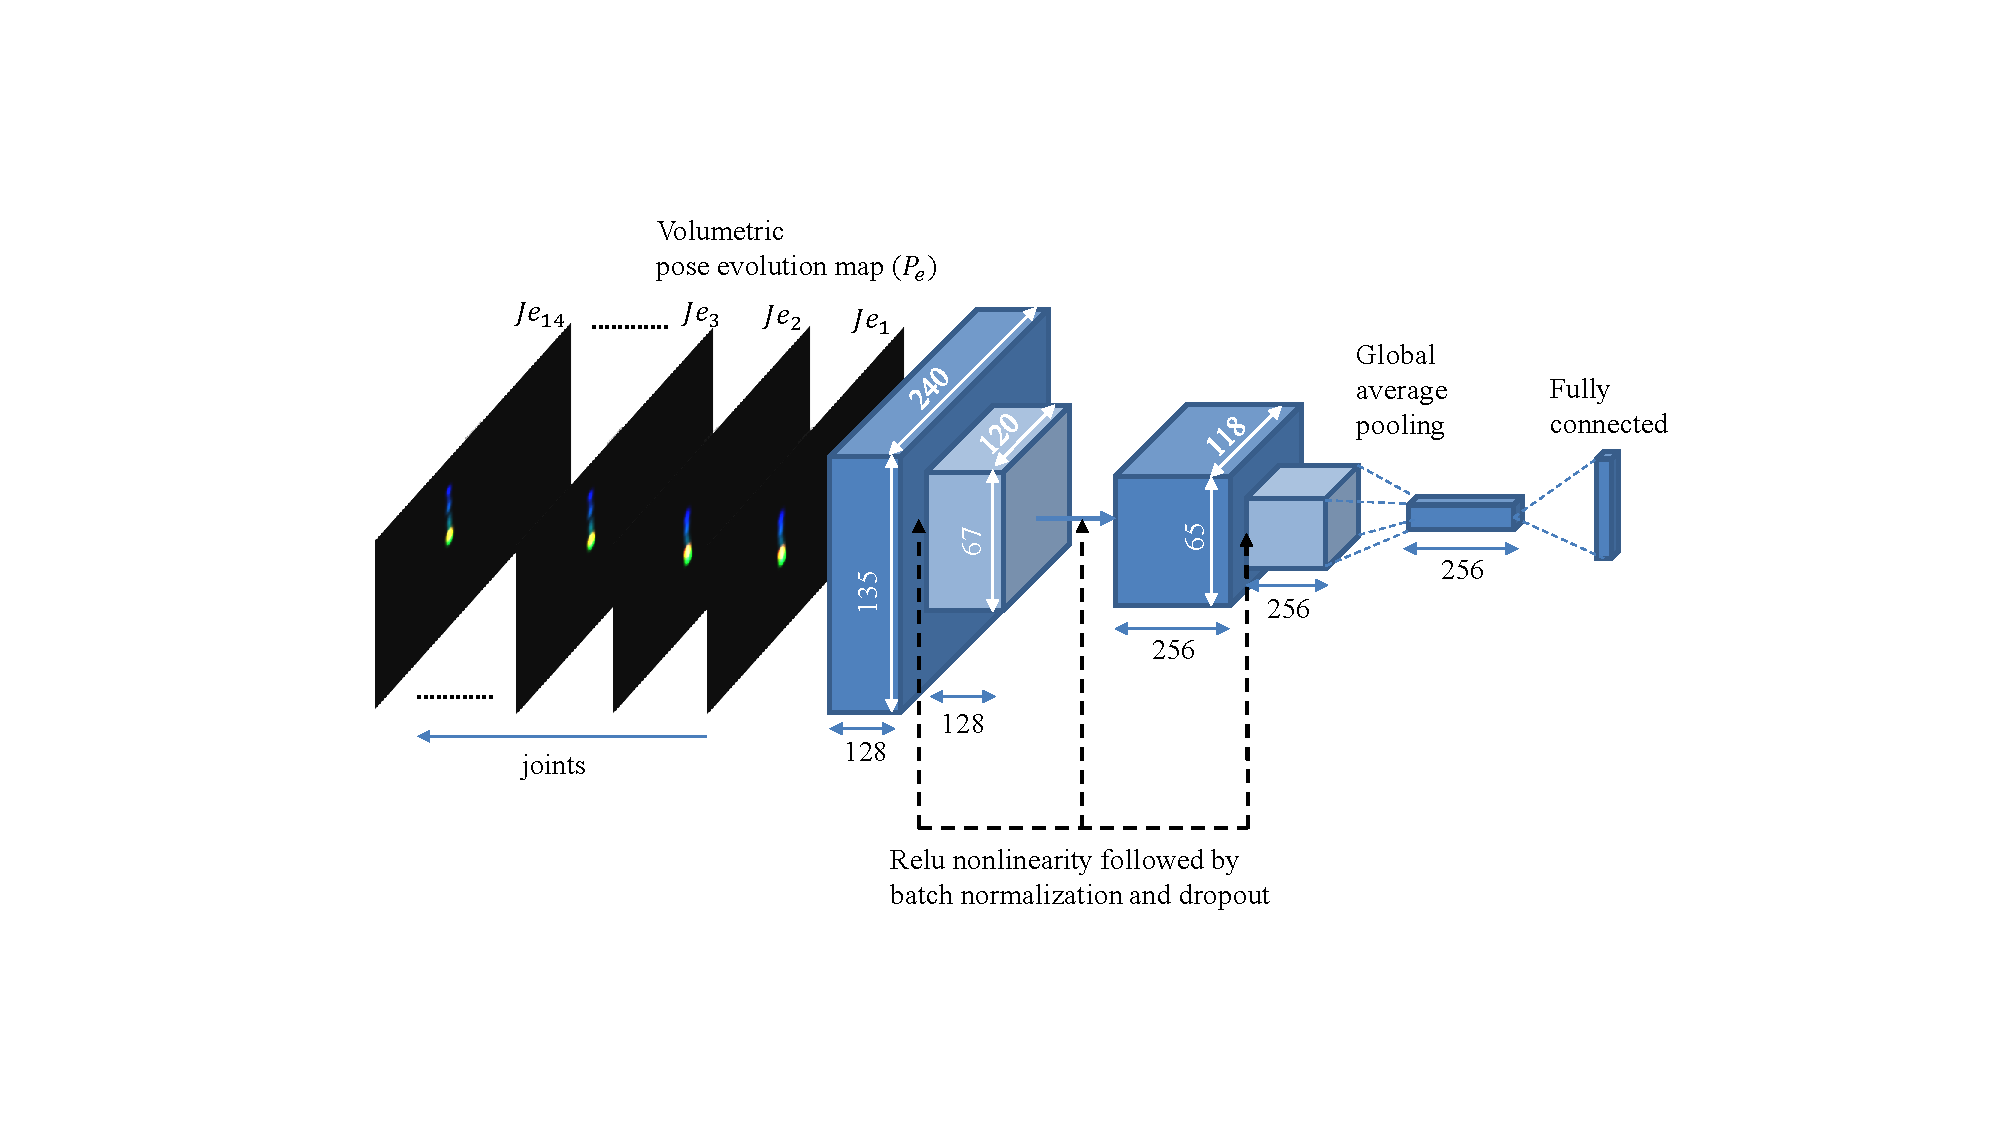
\includegraphics[width=0.5\textwidth, trim=2.1in 1.0in 2.1in 1.0in, clip=true]{Figures/ActionNet.pdf}
    \caption{Architecture of the action classification network. This network takes the volumetric pose evolution map of the target human actor from a video clip as the input and classifies occurrence of an action in the video into one of the five predefined actions (best viewed in color).}
    \label{fig:ActionNet}
    \vspace{-.1in}
\end{figure}
}
%=============================
\newcommand{\ColorCode}{
\begin{figure}[b]
    \centering
    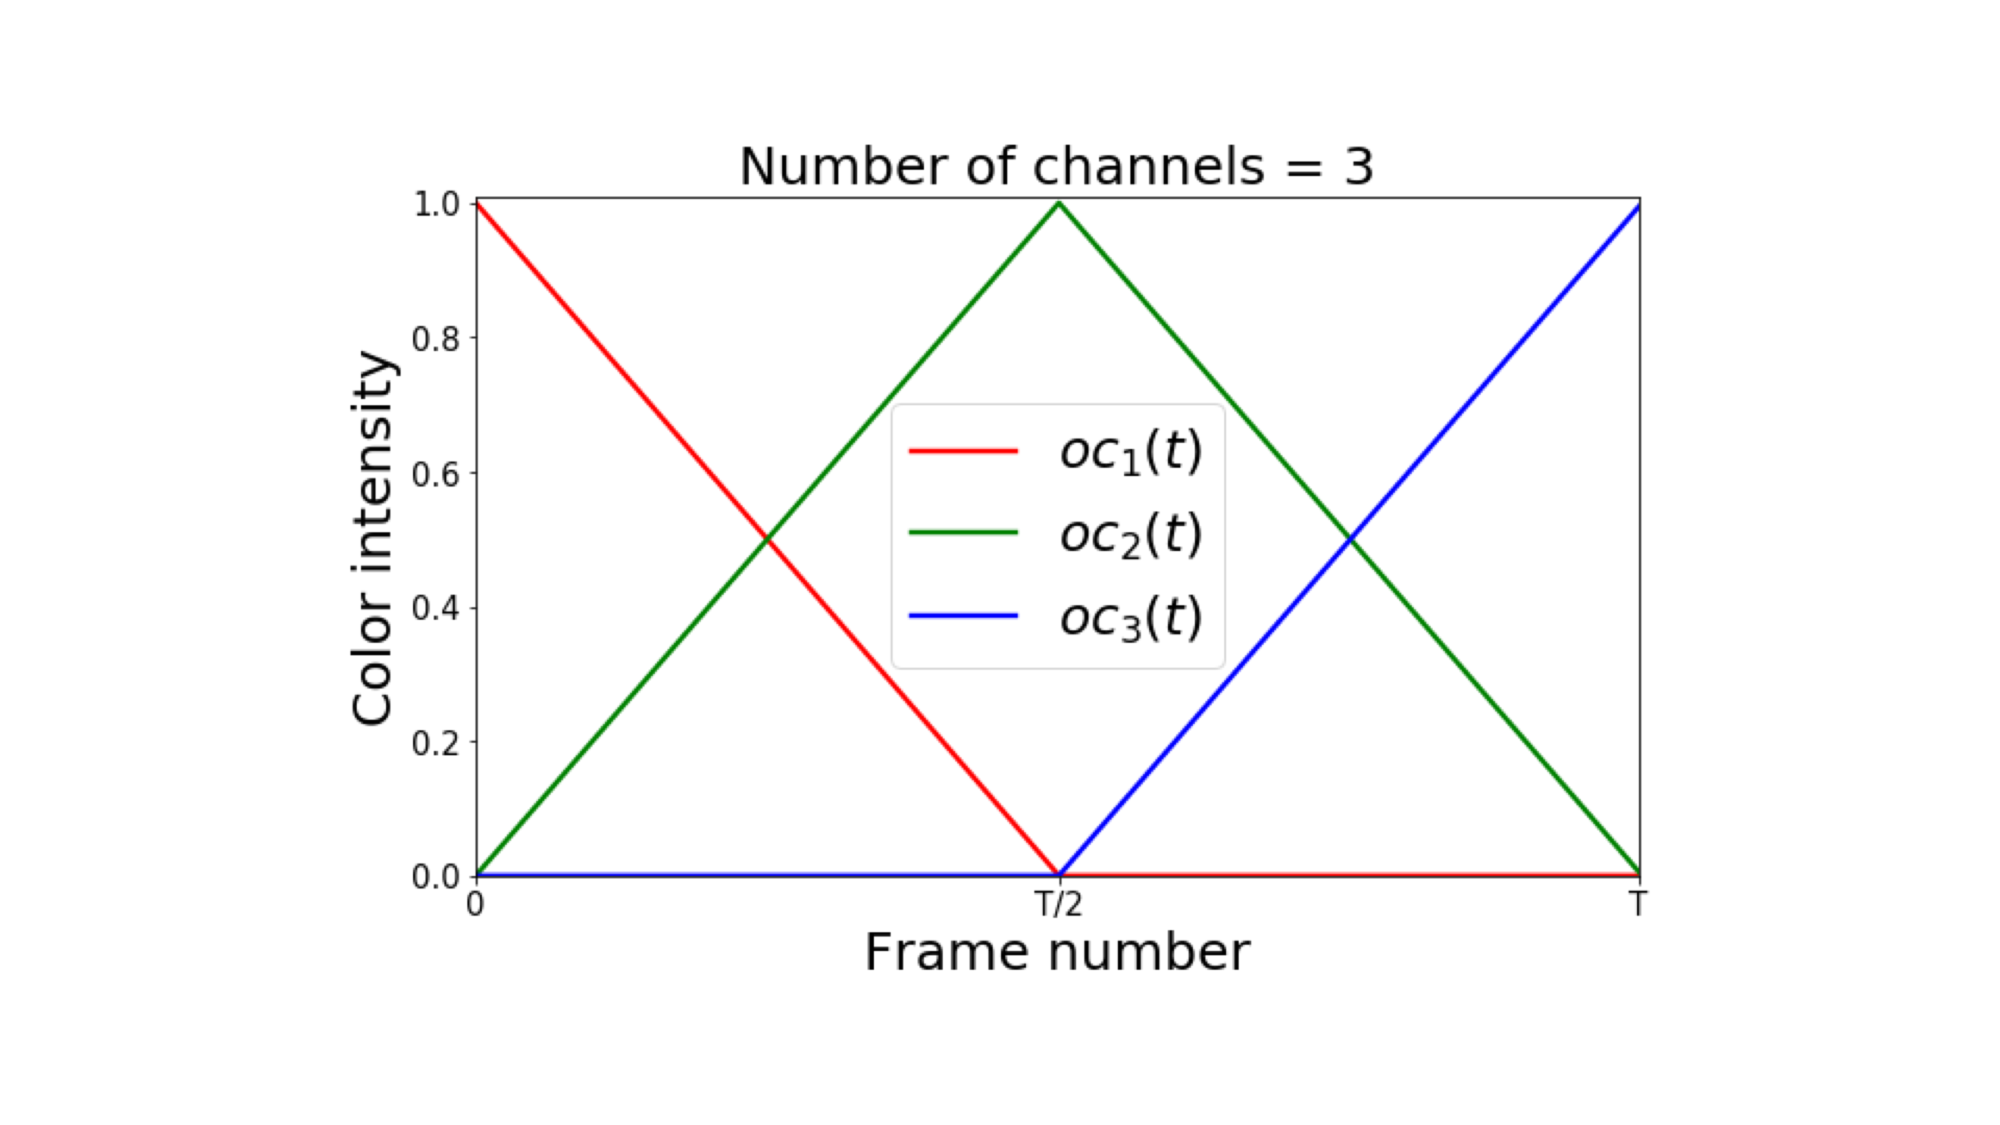
\includegraphics[width=0.27\textwidth, trim=1.9in 0.9in 1.9in 0.9in, clip=true]{Figures/ColorCode.pdf}
    \caption{Demonstration of the time encoded colorization method utilized for creating body pose motion map representation. $oc_1(t)$, $oc_2(t)$, and $oc_3(t)$ show the time encoding function for each color channel.}
    \label{fig:ColorCode}
    \vspace{-.1in}
\end{figure}
}
%===============================
\newcommand{\peseEvolution}{
\begin{figure}[t]
    \centering
    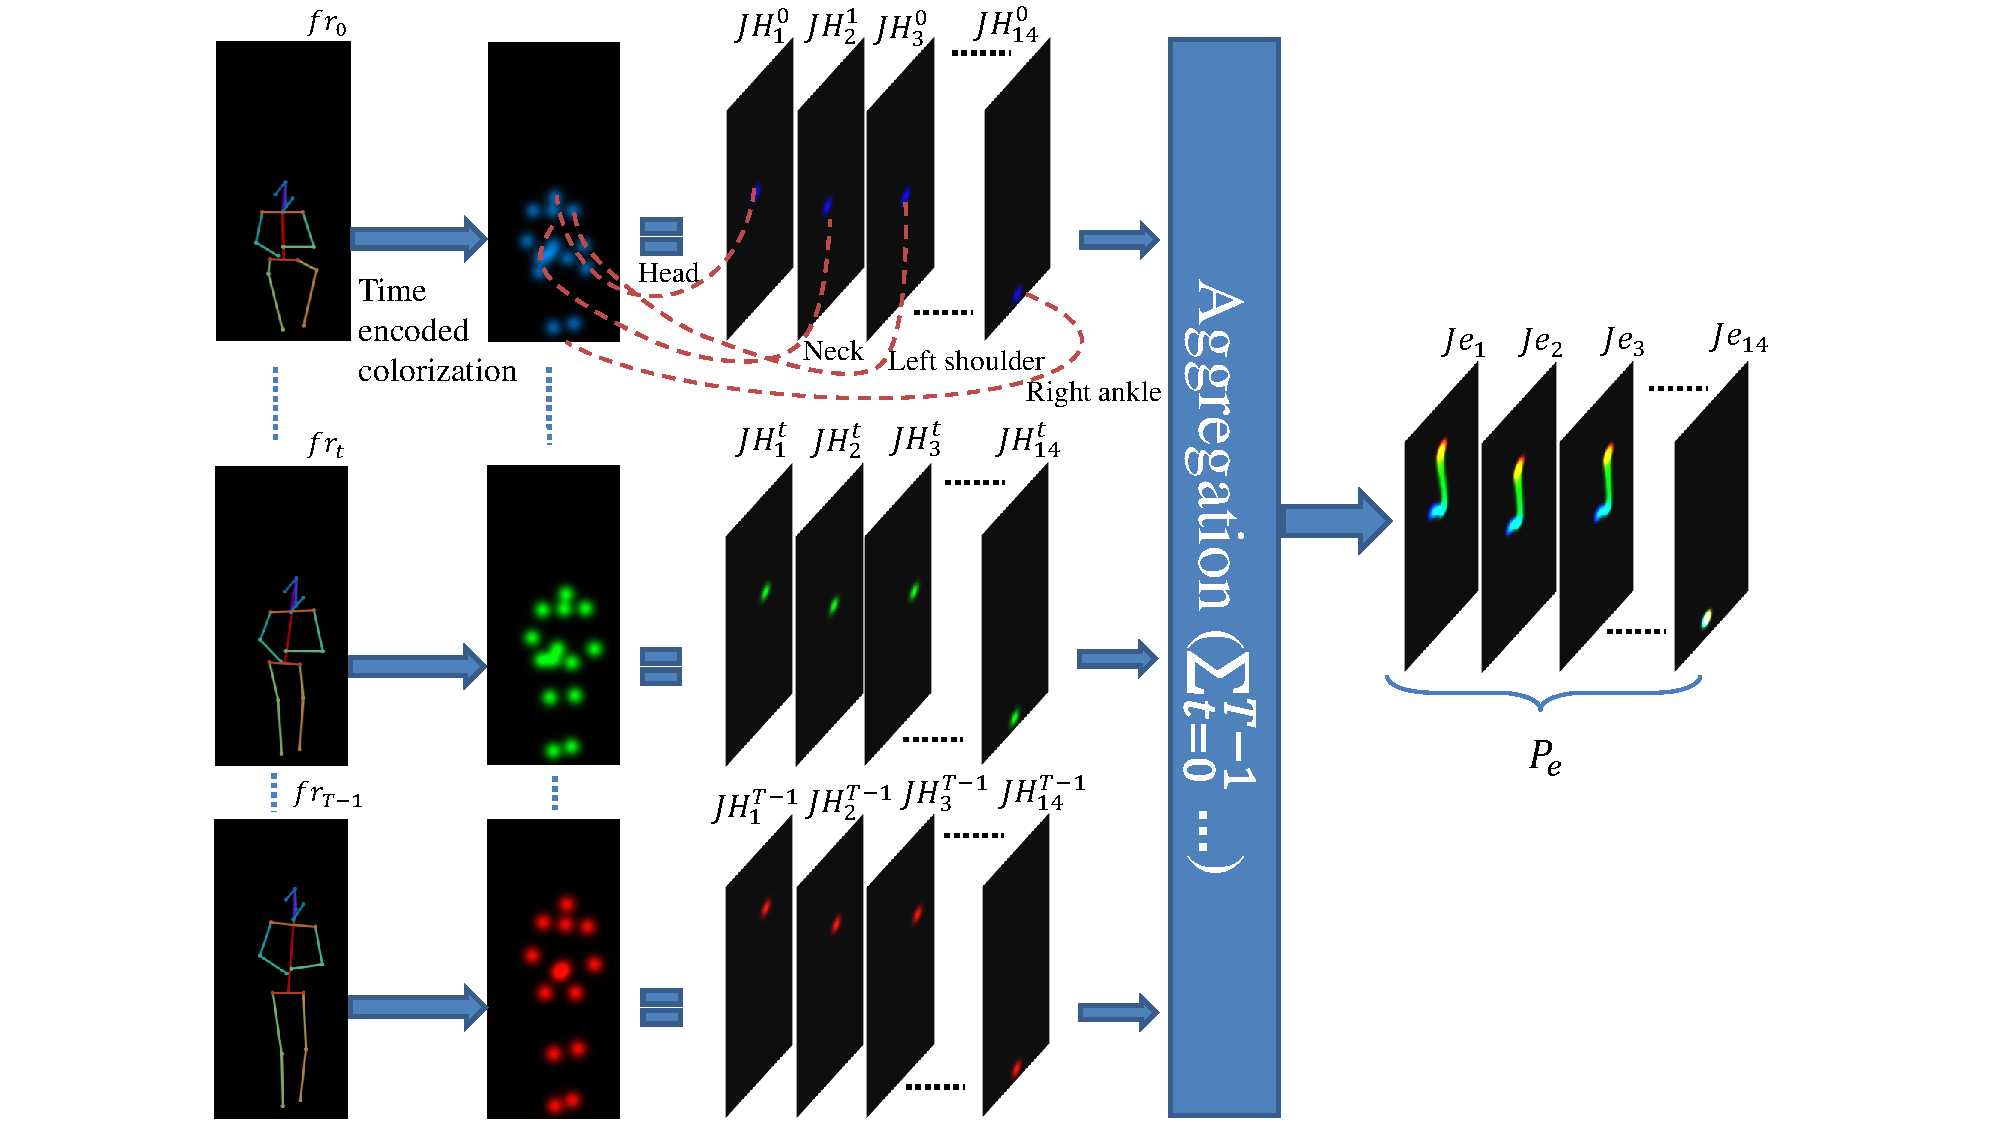
\includegraphics[width=0.5\textwidth, trim=1.0in 0.0in 1.0in 0.0in, clip=true]{Figures/poseEvolution.pdf}
    \caption{Illustration of the pose evolution feature representation in \figref{Method} for the sit-to-stand task. Given the estimated keypoints of the target human actor from preceding stages in the first column, colorized joint heatmaps in the second column are generated using the time encoding function represented in \figref{ColorCode}. The final pose evolution representation is generated by aggregating and normalizing the colorized joint heatmaps in time (best viewed in color).}
    \label{fig:poseEvolution}
%    \vspace{-.1in}
\end{figure}
}
%===============================
\newcommand{\Cmat}{
\begin{figure}[t]
    \centering
    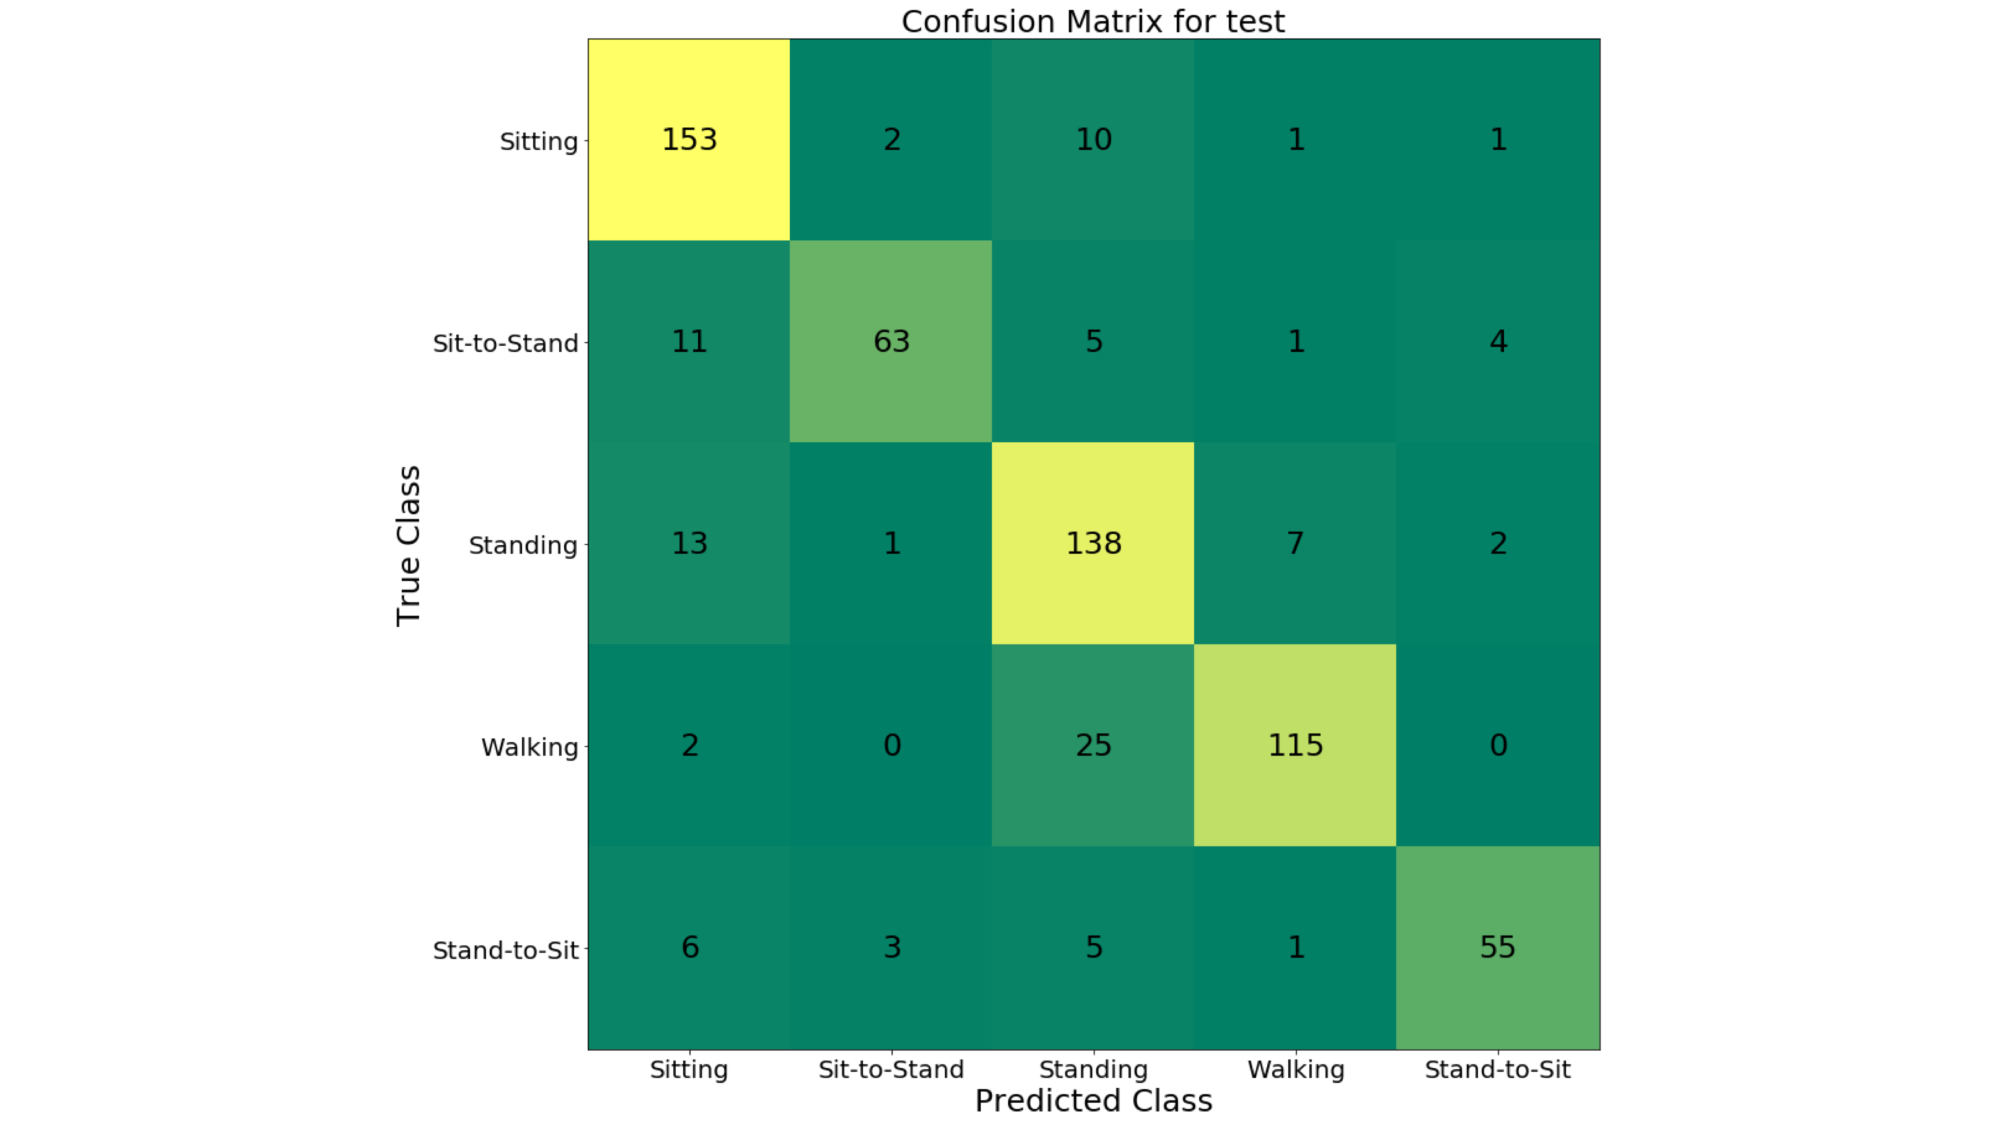
\includegraphics[width=0.35\textwidth, trim=2.5in 0.0in 2.5in 0.0in, clip=true]{Figures/Cmat.pdf}
    \caption{Confusion matrix of the action recognition network evaluated on the test dataset.}
    \label{fig:Cmat}
    \vspace{-.1in}
\end{figure}
}
%=================================
\newcommand{\dataDist}{
\begin{figure}[t]
    \centering
    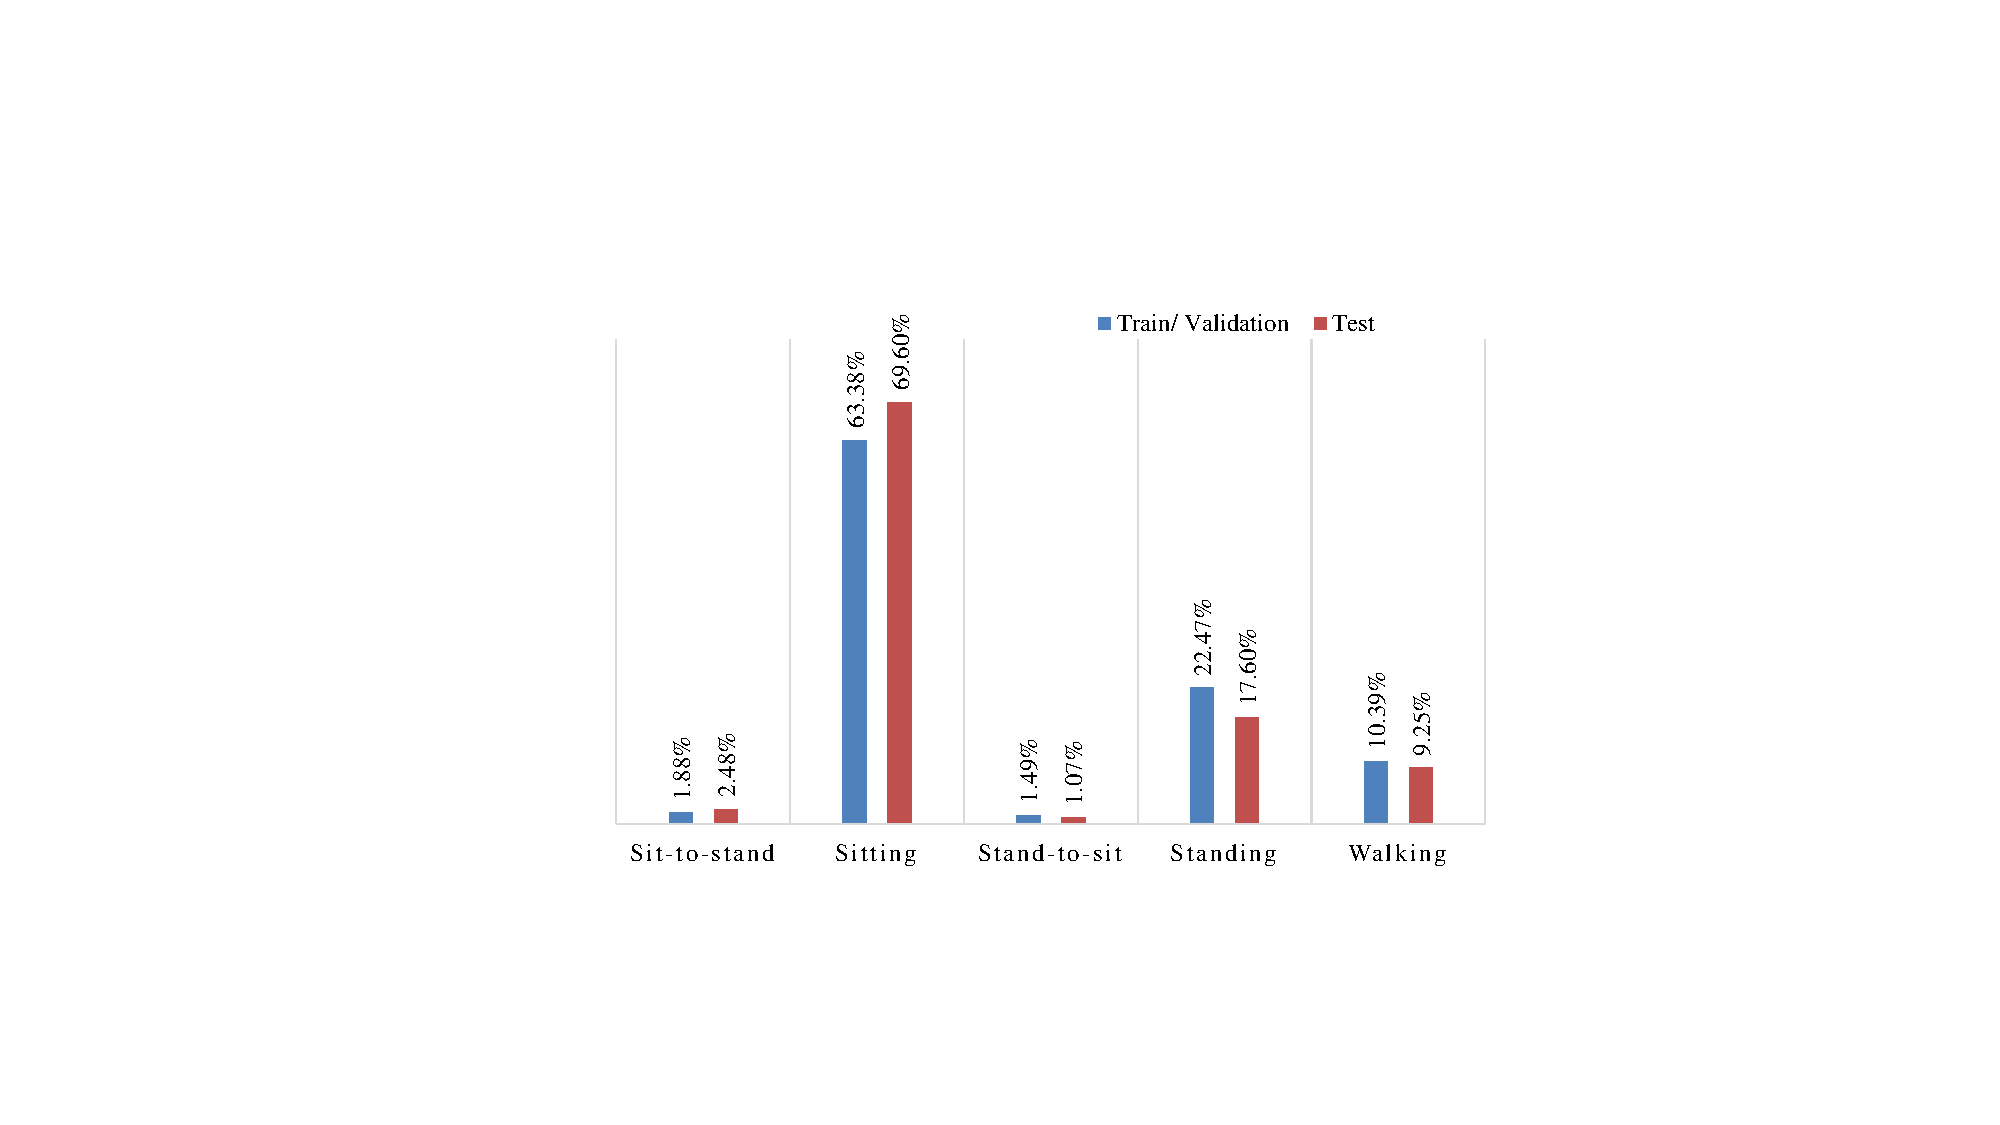
\includegraphics[width=0.4\textwidth, trim=4.1in 1.7in 3.7in 1.8in, clip=true]{Figures/DataDistribution.pdf}
    \caption{Distribution of the action clips based on the type of the actions for test and train/validation datasets. The distribution of the original set of action clips is highly imbalanced. }
    \label{fig:dataDist}
    \vspace{-.1in}
\end{figure}
}
%=================================
\newcommand{\taxonomy}{
\begin{figure}[t]
    \centering
    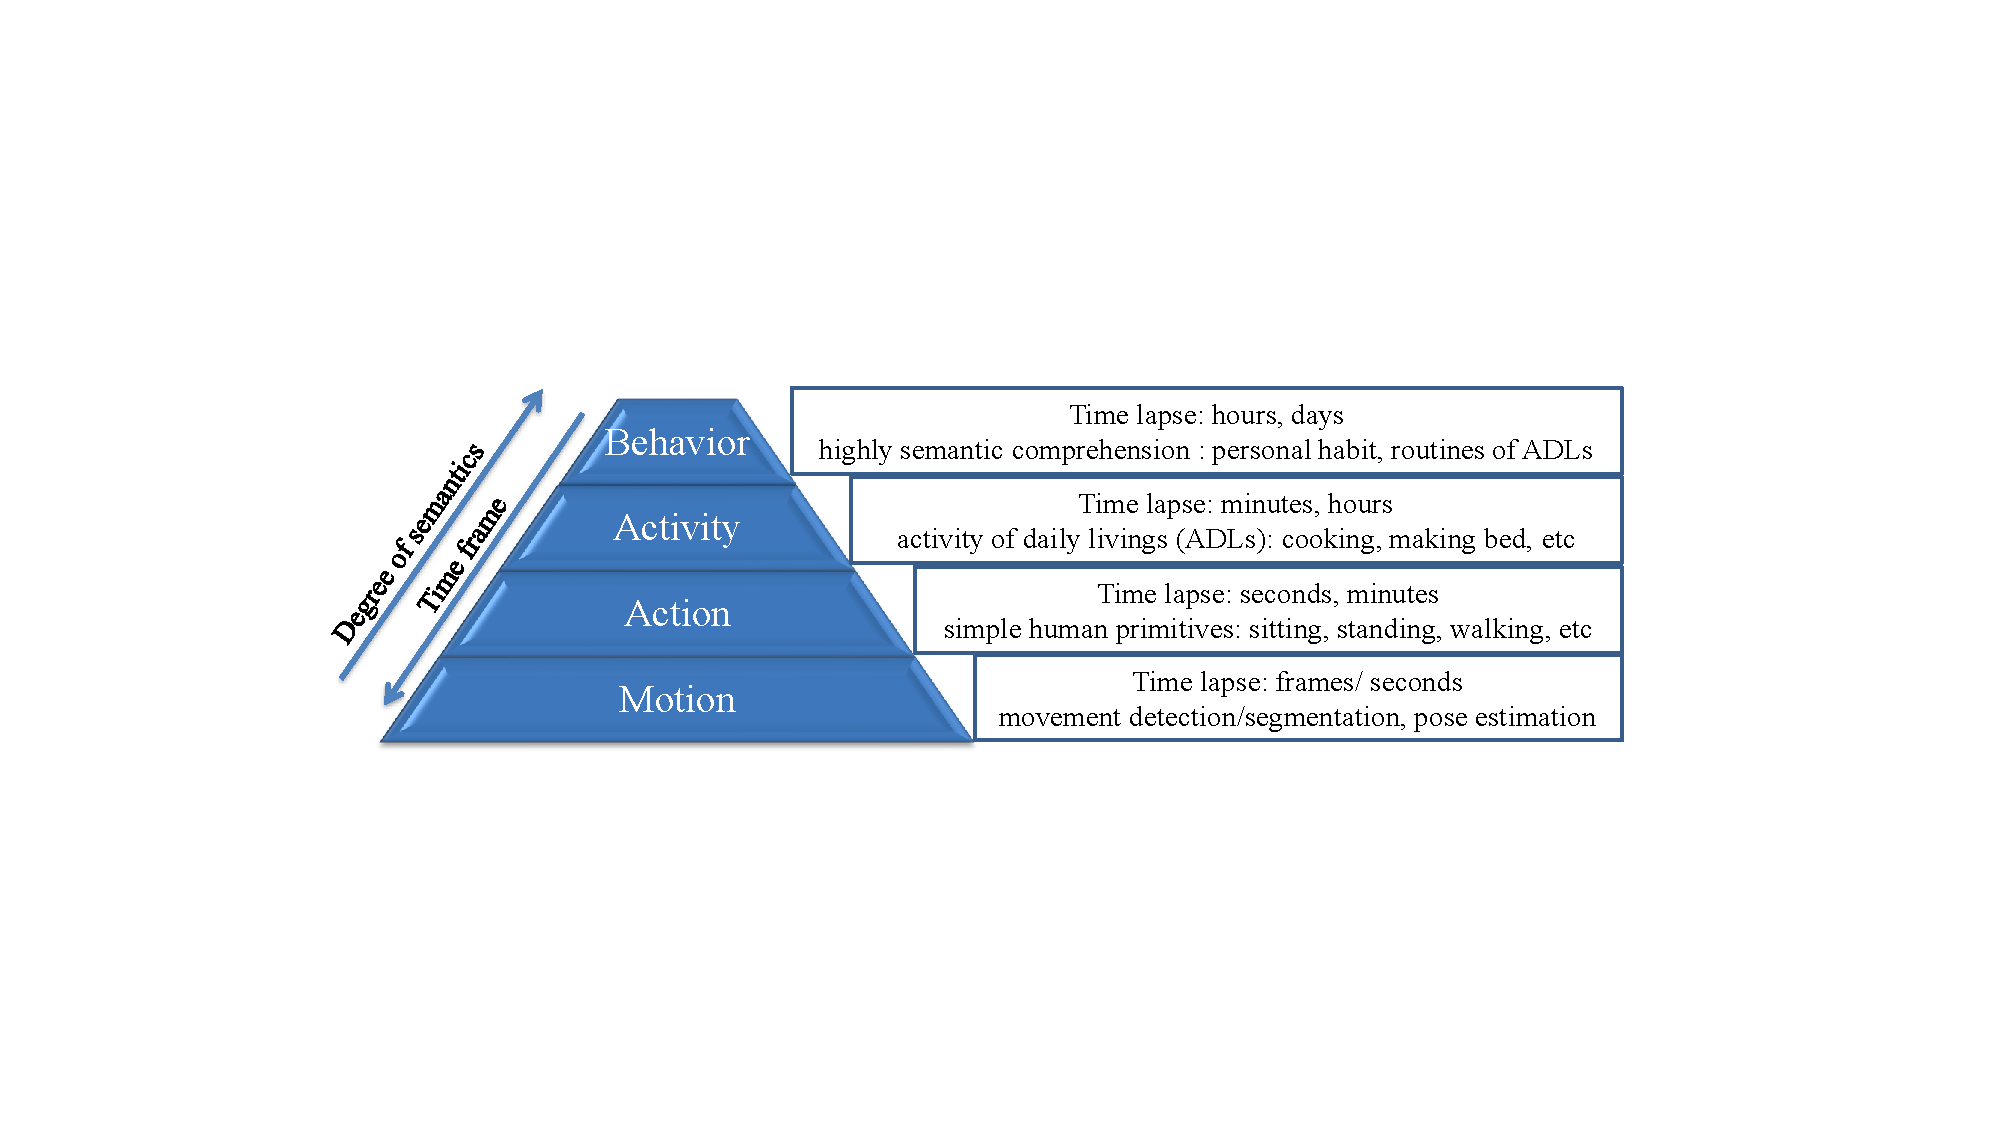
\includegraphics[width=0.5\textwidth, trim=2.2in 2.3in 2.2in 2.3in, clip=true]{Figures/Taxonomy.pdf}
    \caption{Taxonomy of human behaviors with different levels of semantics and complexity. Recognition of each level requires most of the underlying tasks to be recognized \cite{chaaraoui2012review}. }
    \label{fig:taxonomy}
    \vspace{-.1in}
\end{figure}
}

%================================
\newcommand{\chStat}{
\begin{figure}[t]
    \centering
    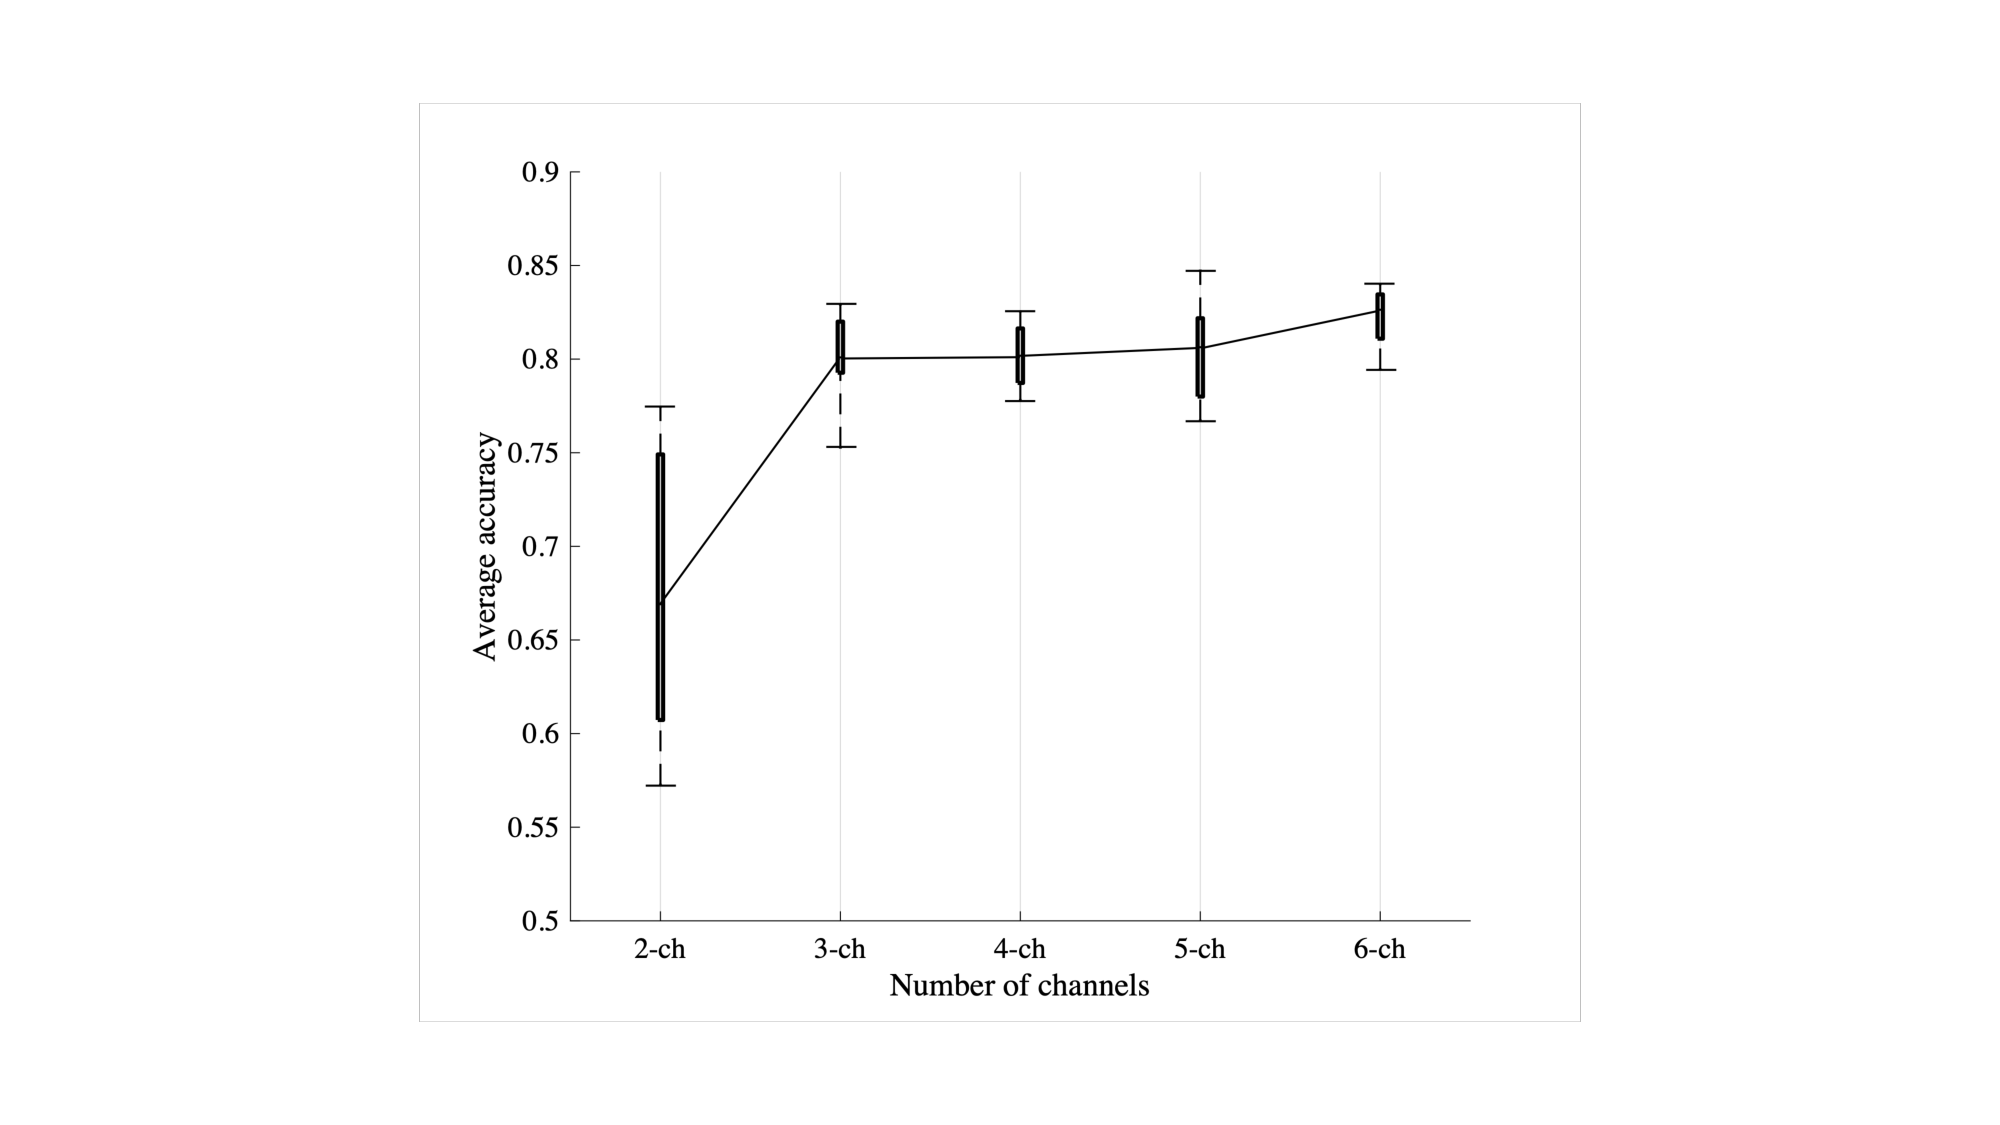
\includegraphics[width=0.35\textwidth, trim=2.7in 0.7in 2.7in 1.0in, clip=true]{Figures/chStat.pdf}
    \caption{Average classification accuracy with respect to the number of channels of input pose evolution representations.}
    \label{fig:chStat}
    \vspace{-.1in}
\end{figure}
}

%====================================

\newcommand{\missclass}{
\begin{figure}[t]
 \centering
  \subfloat[][Standing]{\label{fig:stand}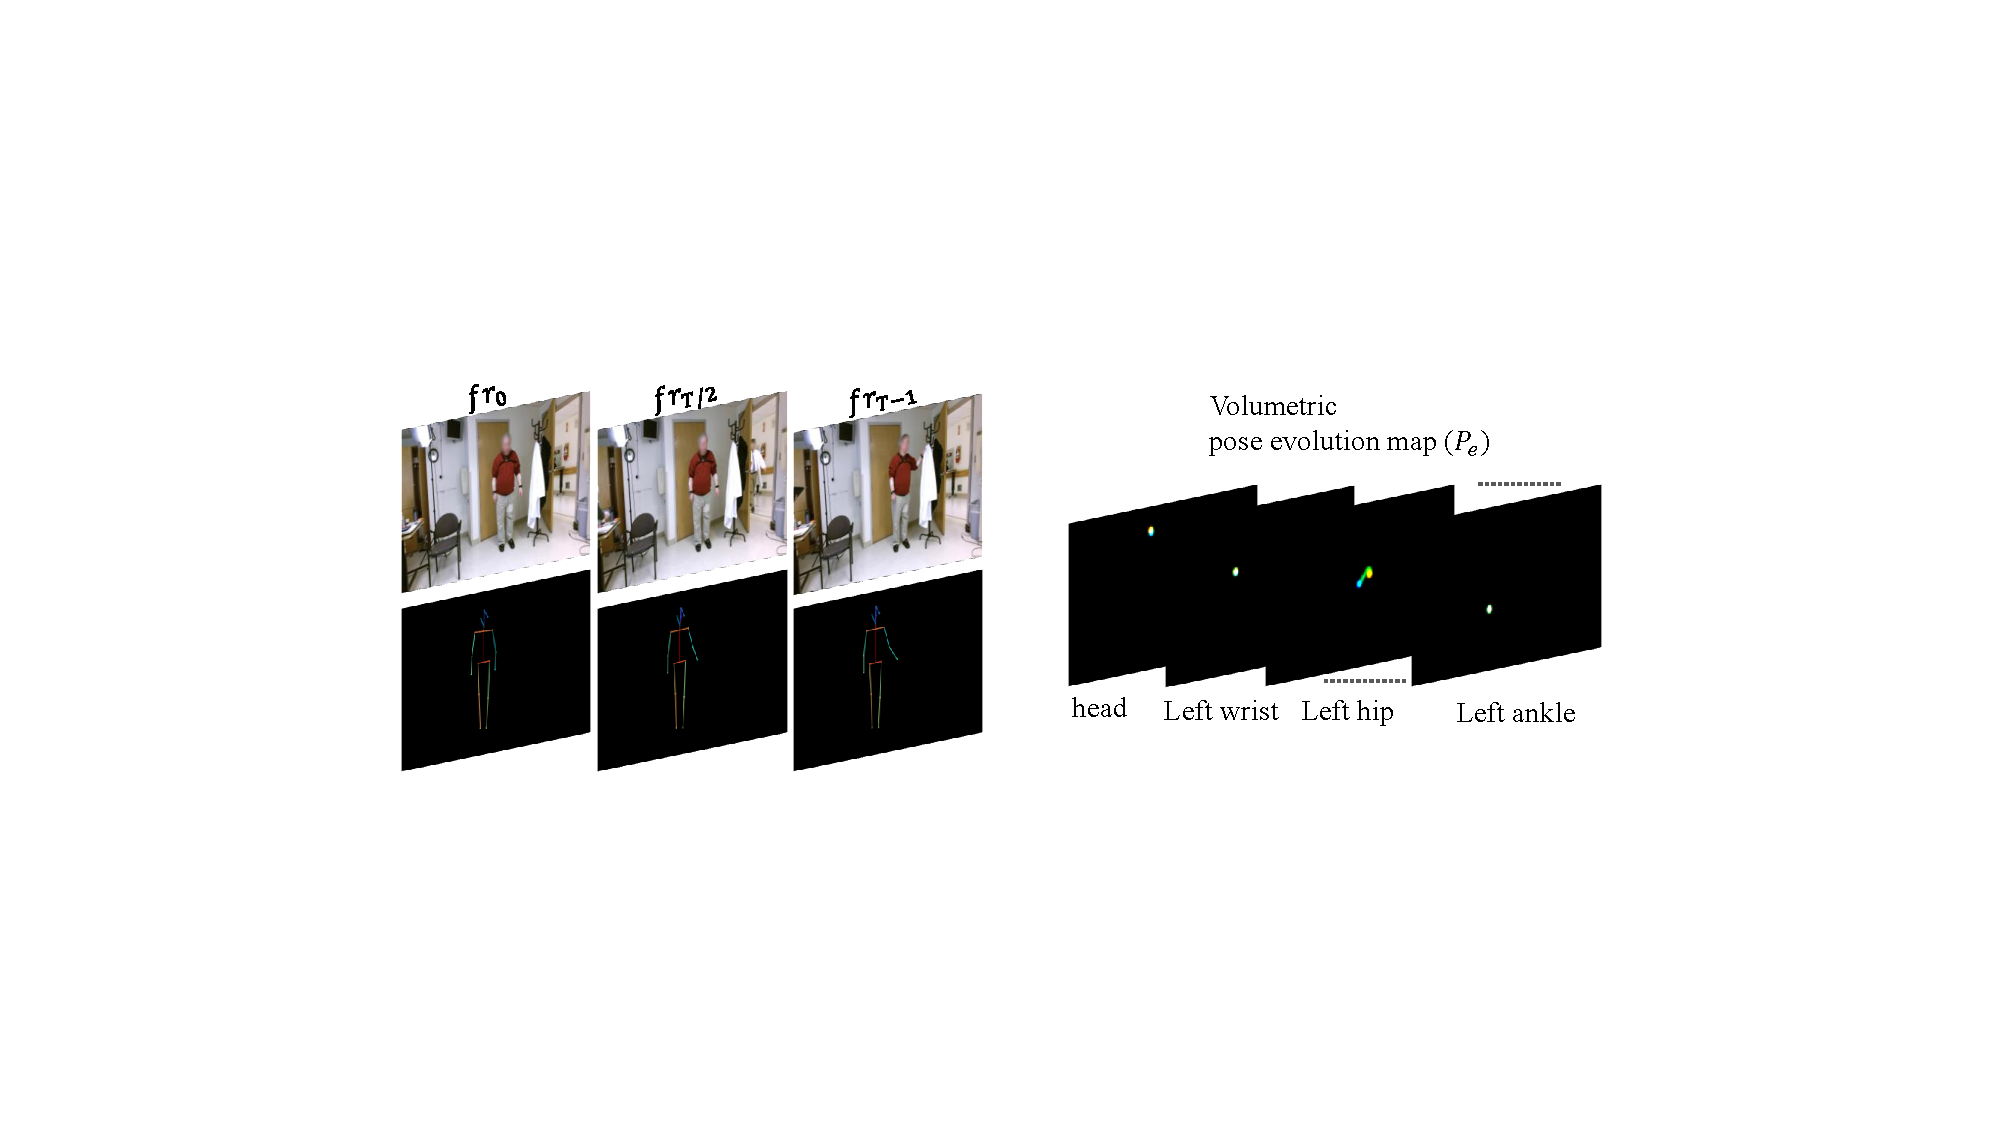
\includegraphics[width=0.5\textwidth, trim=2.5in 2.35in 2.4in 2.5in, clip=true]{Figures/standing.pdf}}\\
  \vspace{-.06in}
 \subfloat[][Transition from standing to walking]{\label{fig:transit}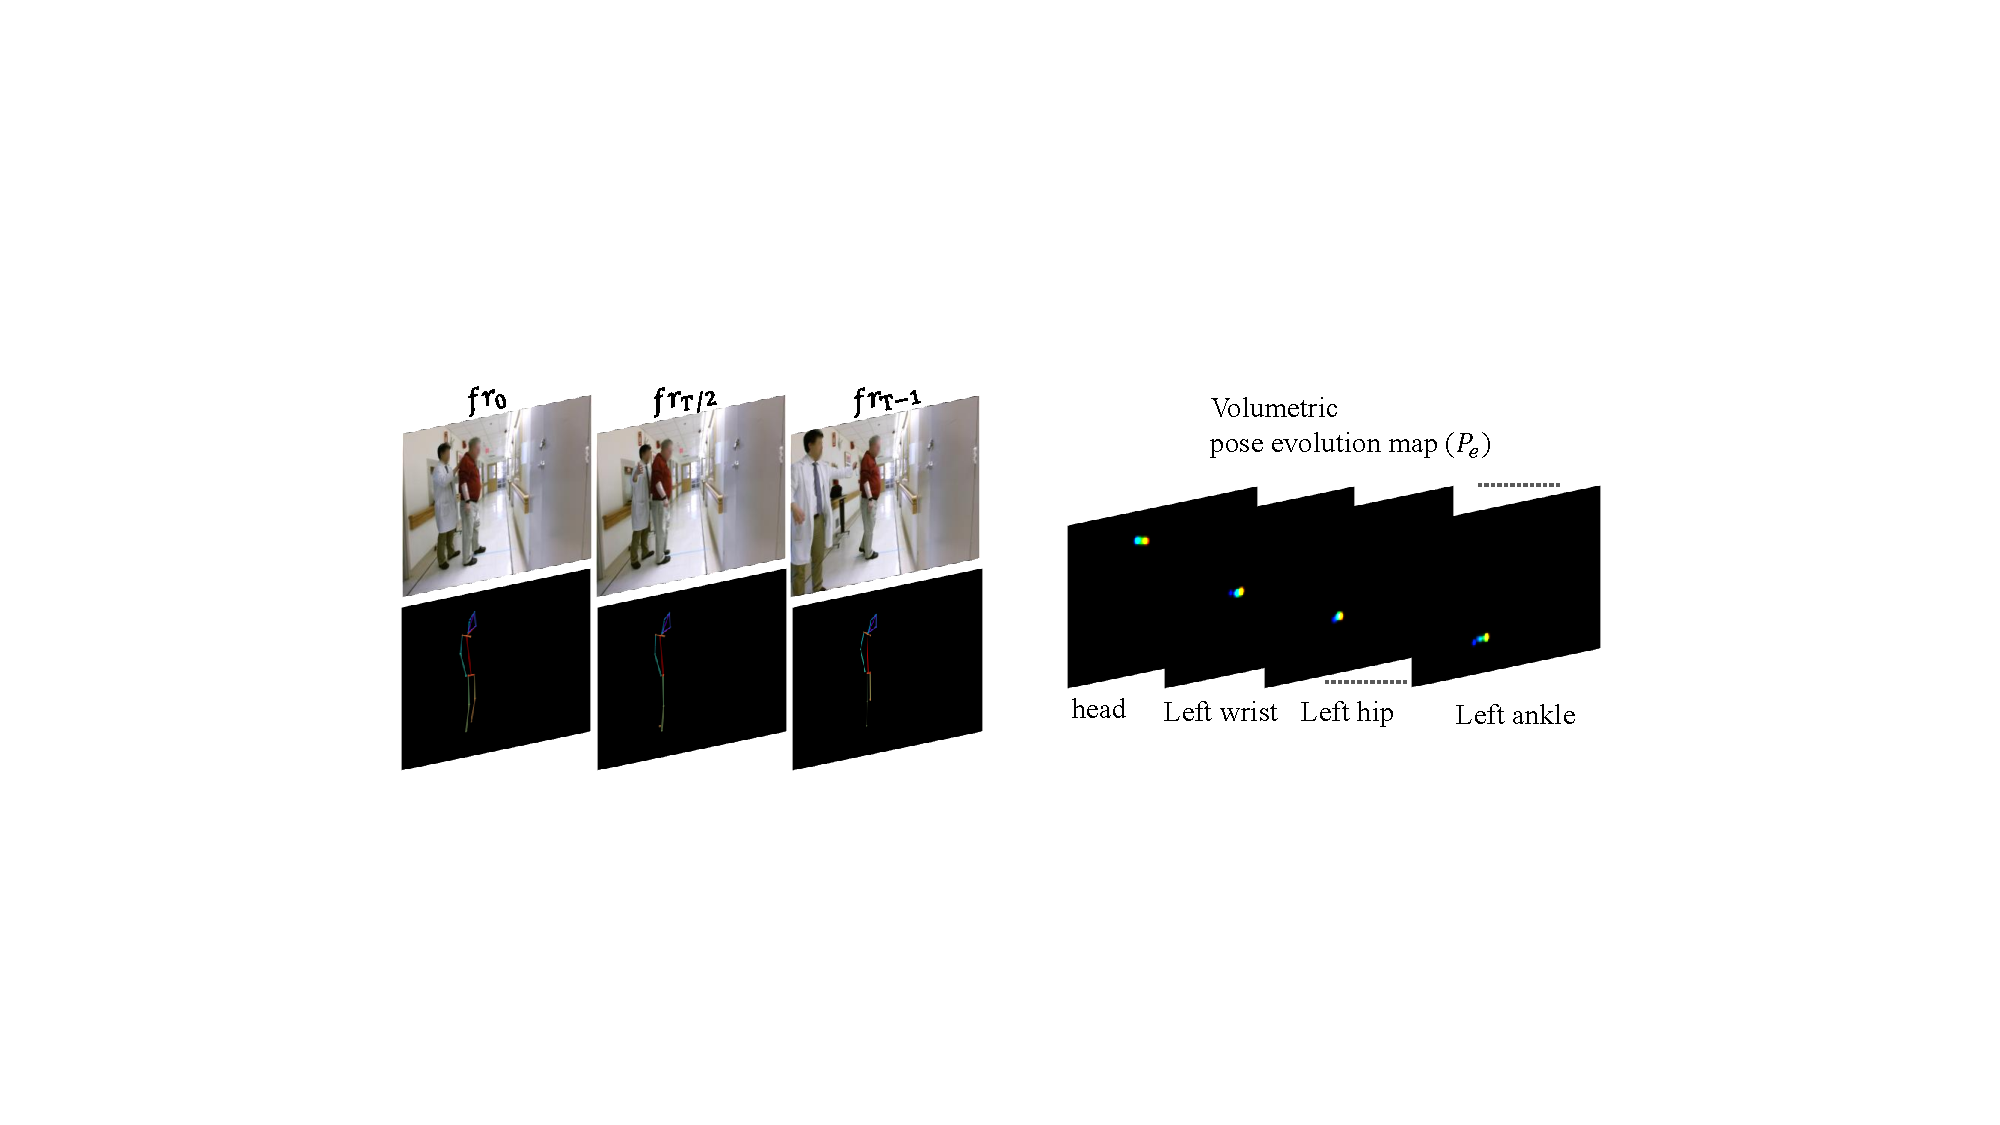
\includegraphics[width=0.5\textwidth, trim=2.5in 2.35in 2.4in 2.5in,
  clip=true]{Figures/transition.pdf}}\\
  \vspace{-.06in}
 \subfloat[][Walking in frontal view]{\label{fig:walk}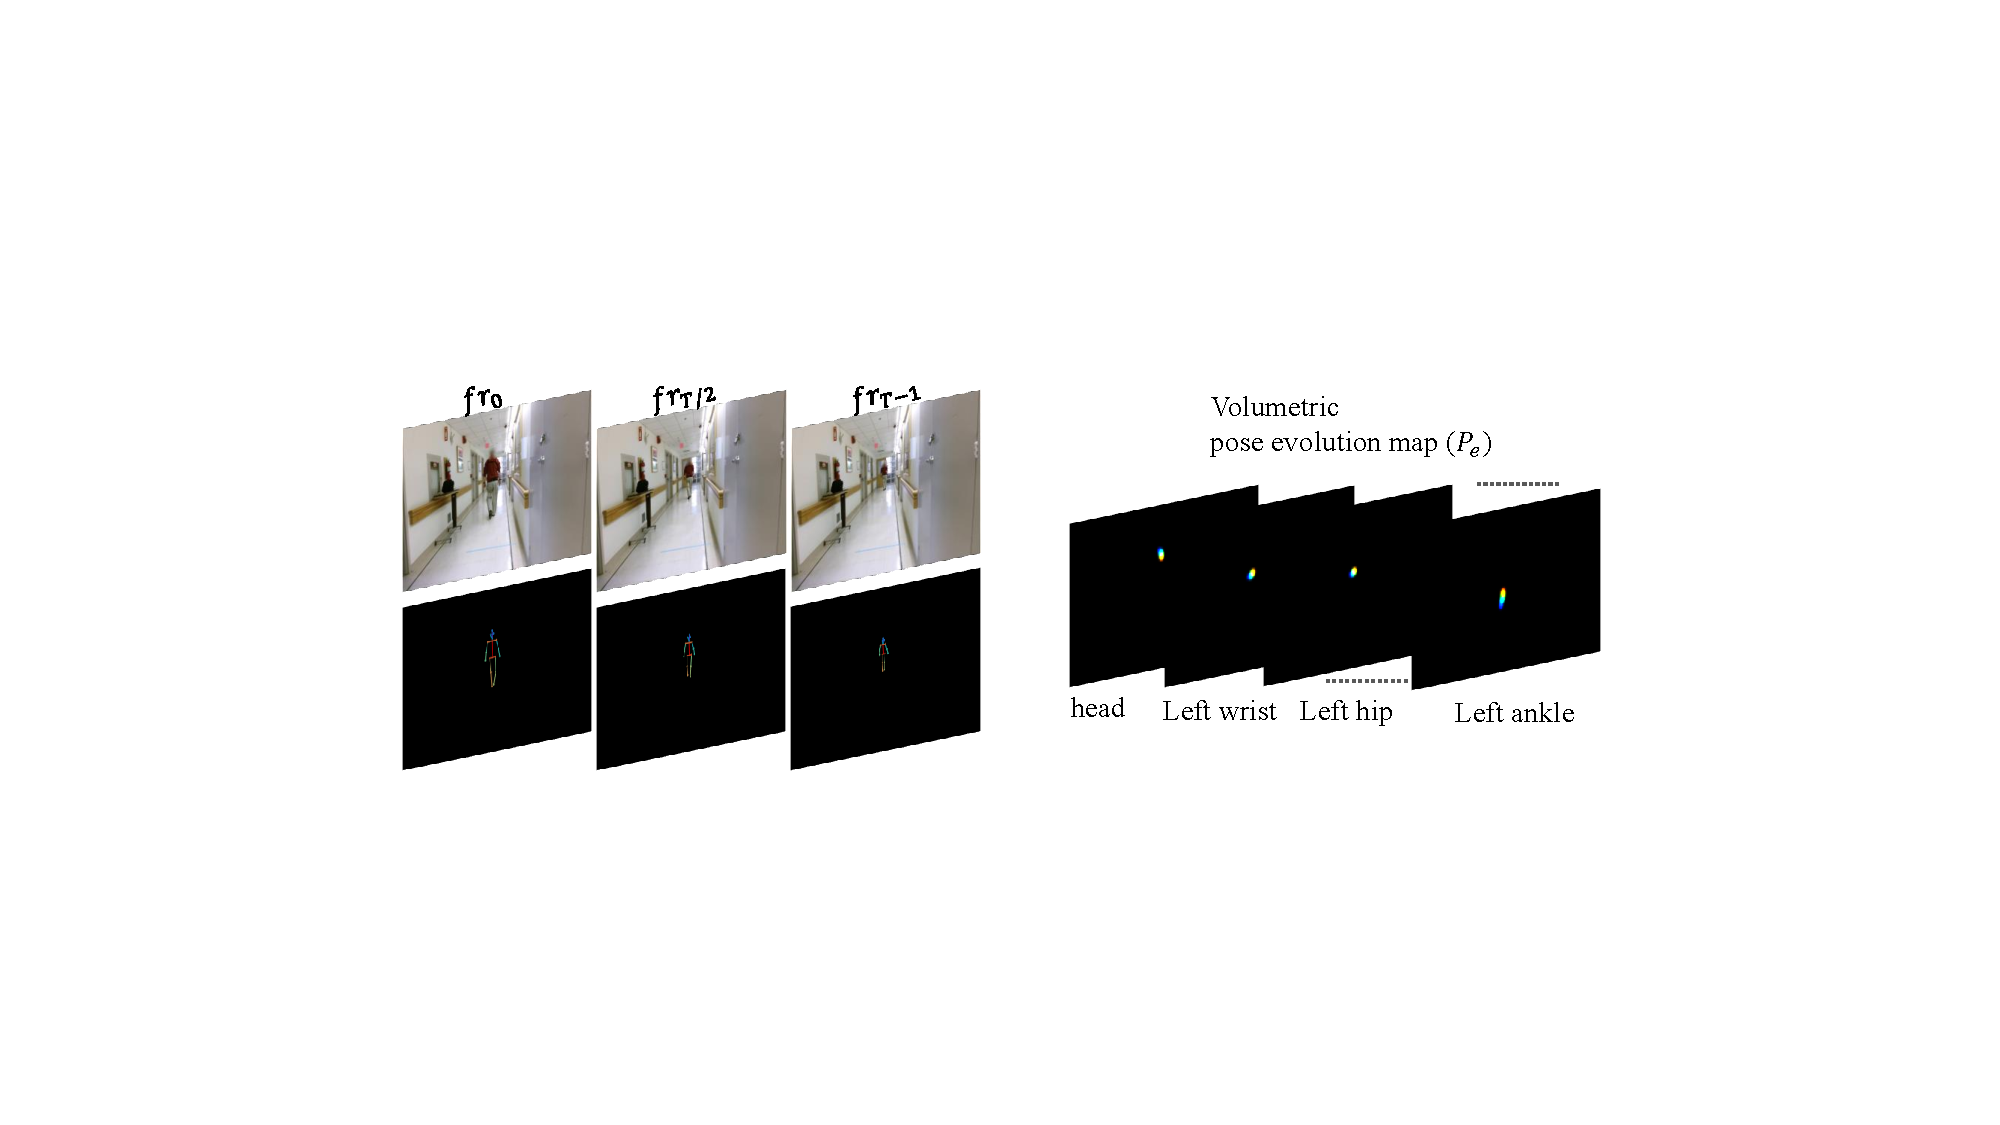
\includegraphics[width=0.5\textwidth,trim=2.5in 2.35in 2.4in 2.5in,
  clip=true]{Figures/walking.pdf}}\\
  \caption{An example of the misclassification of walking as standing. (a), (b), and (c) show the first, middle, and last frame of three action video clips along with the corresponding pose estimations and pose evolution maps. During the manual annotation process (a) was labeled as standing, whereas (b) and (c) were labeled as walking. The action classification network classifies (a) and (b) as standing because they have a very similar pose evolution map (best viewed in color and zoomed in). }
\label{fig:missclass}
\vspace{-.1in}
\end{figure}
}